\begin{exercise}{30}
Consider the following grammar $G = (N, \Sigma, P, S')$, $N=\set{S', S, A}$, $\Sigma=\set{a, b}$ with inherited attributes $i1, i2$ and synthesised attributes $s1, s2$.

\vspace{0.3cm}

  \begin{center}
	$\begin{array}{lcll}
	  S' &\to& S & i1.1 = s1.1 \\
	  &&& i2.1 = 2 \\
	  &&& s1.0 = 1 \\
	  &&& s2.0 = s2.1 \\
	  S &\to& AA & i1.1 = s2.1 \\
	  &&& i2.1 = s1.1 \\
	  &&& i1.2 = 0 \\
	  &&& i2.2 = i2.0 \\
	  &&& s1.0 = s2.1 \\
	  &&& s2.0 = s2.2 \\
	  S &\to& A & i1.1 = 0 \\
	  &&& i2.1 = i2.0 \\
	  &&& s1.0 = 0 \\
	  &&& s2.0 = s2.1 \\
	  A &\to& a & s1.0 = 0 \\
	  &&& s2.0 = i2.0 \\
	  A &\to& b & s2.0 = 0 \\
	  &&& s1.0 = i1.0 \\
	\end{array}$
   \end{center}

\begin{enumerate}[(a)]
  \item Provide the dependency graph for each production in $G$.

  \item Apply the circularity test from the lecture to $G$.

  \begin{enumerate}[1.]
      \item Calculate the set $IS(A)$ for all $A \in N$.
      \item Is $G$ circular? Justify your answer.
  \end{enumerate}

  \item We consider strong noncircularity of $G$.

  \begin{enumerate}[1.]
      \item Calculate the set $IS'(A)$ for all $A \in N$.
      \item Is $G$ strongly noncircular? Justify your answer.
  \end{enumerate}

  \end{enumerate}
\end{exercise}

\begin{solution}

\begin{enumerate}[(a)]
  \item For every production $\pi$ in the attributed grammar, we draw the dependency graph $\rightarrow_\pi$.

\begin{center}
%S'->S
\begin{tikzpicture}[shorten >=1pt,->]
\node (SP) {$S'$};
\node[below of=SP, yshift=-1cm] (S) {$S$};
%\node[left of=SP] (SPi2) {$i_2$};
%\node[left of=SPi2] (SPi1) {$i_1$};
\node[left of=S] (Si2) {$i_2$};
\node[left of=Si2] (Si1) {$i_1$};
\node[right of=SP] (SPs1) {$s_1$};
\node[right of=SPs1] (SPs2) {$s_2$};
\node[right of=S] (Ss1) {$s_1$};
\node[right of=Ss1] (Ss2) {$s_2$};

\path
(SP) edge[dashed] (S)
%(SPi1) edge (Si2)
(Ss2) edge (SPs2)
(Ss1) edge[bend right] (Si1)
;
\end{tikzpicture}
\vspace{3em}

%S->AA
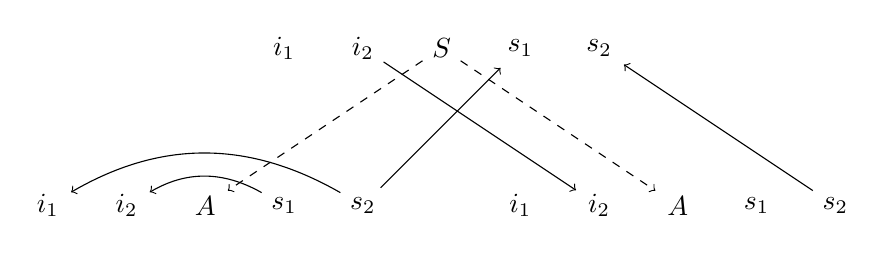
\begin{tikzpicture}[shorten >=1pt,->]
\node (S) {$S$};
\node[left of=S] (Si2) {$i_2$};
\node[left of=Si2] (Si1) {$i_1$};
\node[right of=S] (Ss1) {$s_1$};
\node[right of=Ss1] (Ss2) {$s_2$};

\node[below of=S, xshift=-3cm, yshift=-1cm] (A) {$A$};
\node[left of=A] (Ai2) {$i_2$};
\node[left of=Ai2] (Ai1) {$i_1$};
\node[right of=A] (As1) {$s_1$};
\node[right of=As1] (As2) {$s_2$};

\node[below of=S, xshift=3cm, yshift=-1cm] (A2) {$A$};
\node[left of=A2] (A2i2) {$i_2$};
\node[left of=A2i2] (A2i1) {$i_1$};
\node[right of=A2] (A2s1) {$s_1$};
\node[right of=A2s1] (A2s2) {$s_2$};

\path
(S) edge[dashed] (A)
(S) edge[dashed] (A2)
(Si2) edge (A2i2)
(As1) edge[bend right] (Ai2)
(As2) edge[bend right] (Ai1)
(As2) edge (Ss1)
(A2s2) edge (Ss2)
;
\end{tikzpicture}
\vspace{3em}

%S->A
\begin{tikzpicture}[shorten >=1pt,->]
\node (S) {$S$};
\node[left of=S] (Si2) {$i_2$};
\node[left of=Si2] (Si1) {$i_1$};
\node[right of=S] (Ss1) {$s_1$};
\node[right of=Ss1] (Ss2) {$s_2$};

\node[below of=S, yshift=-1cm] (A) {$A$};
\node[left of=A] (Ai2) {$i_2$};
\node[left of=Ai2] (Ai1) {$i_1$};
\node[right of=A] (As1) {$s_1$};
\node[right of=As1] (As2) {$s_2$};

\path
(S) edge[dashed] (A)
(Si2) edge (Ai2)
(As2) edge (Ss2)
;
\end{tikzpicture}
\hfill
%A->a
\begin{tikzpicture}[shorten >=1pt,->]
\node (A) {$A$};
\node[left of=A] (Ai2) {$i_2$};
\node[left of=Ai2] (Ai1) {$i_1$};
\node[right of=A] (As1) {$s_1$};
\node[right of=As1] (As2) {$s_2$};

\node[below of=S, yshift=-1cm] (a) {$a$};

\path
(A) edge[dashed] (a)
(Ai2) edge[bend right] (As2)
;
\end{tikzpicture}
\hfill
%A->b
\begin{tikzpicture}[shorten >=1pt,->]
\node (A) {$A$};
\node[left of=A] (Ai2) {$i_2$};
\node[left of=Ai2] (Ai1) {$i_1$};
\node[right of=A] (As1) {$s_1$};
\node[right of=As1] (As2) {$s_2$};

\node[below of=S, yshift=-1cm] (b) {$b$};

\path
(A) edge[dashed] (b)
(Ai1) edge[bend right] (As1)
;
\end{tikzpicture}
\end{center}

\item
\begin{enumerate}[1.]
    \item $IS(A)=\{is_1, is_2\}$
    where
    \begin{itemize}
        \item $is_1 = is[A\rightarrow a]=\set{(i_2, s_2)}$
        \item $is_2 = is[A\rightarrow b]=\set{(i_1, s_1)}$
    \end{itemize}
    $IS(S)=\{is_3, \ldots, is_8\}=\set{is_3, \emptyset)}$
    where
    \begin{itemize}
        \item $is_3 = is[S\rightarrow A, is_1] = \set{(i_2, s_2)}$
        \item $is_4 = is[S\rightarrow A, is_2] = \emptyset$
        \item $is_5 = is[S\rightarrow A\,A, is_1, is_1] = \set{(i_2, s_2)}$
        \item $is_6 = is[S\rightarrow A\,A, is_1, is_2] = \emptyset$
        \item $is_7 = is[S\rightarrow A\,A, is_2, is_1] = \set{(i_2, s_2)}$
        \item $is_8 = is[S\rightarrow A\,A, is_2, is_2] = \emptyset$
    \end{itemize}
    $IS(S')=\{is_9, is_10\}$
    where
    \begin{itemize}
        \item $is_9 = is[S'\rightarrow S, \emptyset] = \emptyset$
        \item $is_10 = is[S'\rightarrow S, is_3] = \emptyset$
    \end{itemize}

\item G is not circular.
    There are three possible cover productions, $S' \rightarrow S$, $S \rightarrow A$ and $S \rightarrow AA$.
    \begin{itemize}
    \item $S' \rightarrow S$: We only have the cover $(s_1, i_1)$ for $S$, but since $(i_1, s_1) \not \in \set{(i_2, s_2)}$ and $(i_1, s_1) \not \in \emptyset$, the relations are non cyclic.
    \item $S \rightarrow A$: No cover relation
    \item $S \rightarrow AA$: We only have the cover relation $\set{(s_1, i_2), (s_2, i_1)}$ for $A$, however for
    \begin{itemize}
        \item for $is_1 = \set{(i_2, s_2)}$ we have the relation $\set{(s_1, i_2), (s_2, i_1)} \cup \set{(i_2, s_2)}$, which is non cyclic and
       \item for $is_2 = \set{(i_1, s_1)}$ we have the relation $\set{(s_1, i_2), (s_2, i_1)} \cup \set{(i_1, s_1)}$, which is not cyclic as well.
    \end{itemize}
    \end{itemize}
    Therefore it is impossible to construct a dependency graph with a cycle.
\end{enumerate}

\item
\begin{enumerate}[1.]
    \item For each non-terminal $A$ we compute the $IS'$ sets by $IS'(A) = \bigcup \set{is \mid is \in IS(A)}$.
    \begin{align*}
        IS'(A) &= is_1 \cup is_2 = \set{(i_1, s_1),(i_2, s_2)} \\
        IS'(S) &= \emptyset \cup is_3 = \set{(i_2, s_2)} \\
        IS'(S') &= \emptyset
    \end{align*}

    \item The grammar is \emph{not} strongly noncircular as we can construct a cycle by taking the production $S \to A\,A$ and using the dependencies in $IS'(A)$.
        This gives us the cycle $i_1 \rightarrow s_1 \rightarrow i_2 \rightarrow s_2 \rightarrow i_1$.
\end{enumerate}
\end{enumerate}
\end{solution}
